\documentclass[11pt]{article}
%\documentclass{book}
\usepackage[utf8]{inputenc}
\usepackage[T1]{fontenc}
\usepackage[french]{babel}
\usepackage[top=1.8cm, bottom=1.8cm, left=1.8cm, right=1.8cm]{geometry}
\usepackage[linktocpage,colorlinks=false]{hyperref}
\usepackage{graphicx}
\usepackage{epsfig}
\usepackage{amssymb}
\usepackage{amsmath}
\usepackage{array}
\usepackage{subfig}
\usepackage{multicol}
\usepackage{caption}
\usepackage{listings}
\usepackage{algorithm}
\usepackage{algorithmic}
\hypersetup{
    colorlinks=true,
    breaklinks=true,
    urlcolor=red,
}
\parskip=5pt

\title{\huge{\textbf Spécifications}}
\author{AYOUB Pierre, BASKEVITCH Claire, BESSAC Tristan, \\
CAUMES Clément, DELAUNAY Damien, DOUDOUH Yassin}
\date{Mercredi 18 Avril 2018}

\begin{document}

\maketitle
\vspace{20em}
\begin{center}
\includegraphics{pictures/Application.png}\end{center}
\newpage

\tableofcontents

\newpage

\section{Introduction}

En réalisant le cahier des charges concernant l'application StegX, 
l'analyse des contraintes et des besoins du client nous amène à rédiger 
les spécifications. 

Le logiciel StegX pourra proposer de cacher des données dans des fichiers 
dont le format est pris en charge par l'application. De plus, un utilisateur 
pourra extraire les données cachées d'un fichier qu'on considère déjà comme 
hôte. StegX prendra en charge les trois algorithmes de stéganographie suivants : 
EOF, LSB et MetaData. 

Avec l'analyse des fonctionnalités de l'application, nous avons vu qu'elle 
devait gérer la manipulation de données binaires et donc il fallait un 
langage proche de la machine. 
De plus, nous devons implémenter des fonctions de stéganographie afin de 
cacher des données dans des fichiers. Par conséquent, une programmation 
procédurale était nécessaire. 
Enfin, il fallait des structures ou des objets simples afin de manipuler 
des structures de fichiers. 
De ce fait, nous avons choisi le langage C pour implémenter la future 
application StegX. En effet, le langage C propose une programmation procédurale, 
ainsi qu'un langage bas niveau proche de la machine. Enfin, la possibilité 
d'écriture et de lecture de bits et d'accès mémoire avec le langage C correspond 
à nos besoins. 
C'est donc pour toutes ces raisons que l'équipe de conception de StegX a 
choisi le langage C pour implémenter l'application. 

Après l'étude des différents modules de l'organigramme, ainsi que les informations 
qui se déplacent, nous avons établi un organigramme. 
Cet organigramme nous permettra ainsi de rédiger en détail les spécifications 
des différents modules de l'application. 

\section{Modules du produit}
\subsection{Organigramme}

\hspace{1cm}
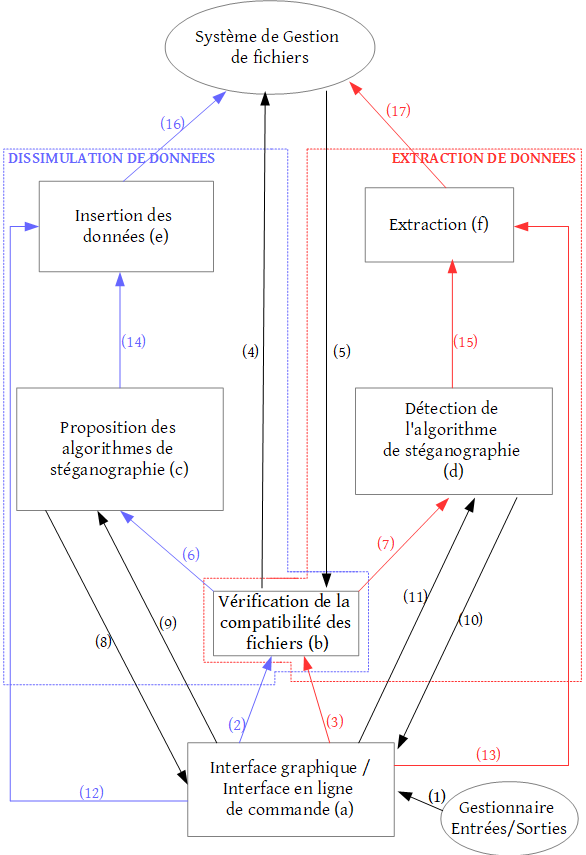
\includegraphics[scale=0.71]{pictures/organigramme.png}

\subsection{Liste des modules et de leurs fonctionnalités}

\begin{description}
\item[a)] \textbf{Interface graphique / Interface en ligne de commande} :
    interfaces permettant à l'utilisateur de choisir parmi les deux
    fonctionnalités possibles de l'application. Il peut dissimuler des
    données dans un fichier (dont le type et le format sont pris en charge
    par l'application). Ou bien, il peut extraire les données cachées d'un
    fichier. \newline
    Il aura donc un mécanisme pour choisir le fichier hôte et le fichier 
    à cacher (pour la dissimulation de données), et un mécanisme pour choisir le 
    fichier contenant les données cachées à analyser (pour l'extraction de 
    données cachées), grâce à une interaction avec le gestionnaire Entrée/Sorties. 

\item[b)] \textbf{Vérification de la compatibilité des fichiers} : le format 
	du fichier hôte (pour le module \textit{Dissimulation de données}) ou 
	le format du fichier à analyser (pour le module \textit{Extraction de données 
	cachées}), choisis par l'utilisateur, est vérifié pour savoir s'il est 
	bien pris en charge par l'application. \newline
	Il aura un mécanisme de lecture du fichier hôte : selon les formats 
	pris en charge, il y aura une batterie de tests pour déterminer le 
	format du fichier. 
	Il prendra en entrée les chemins de fichiers en entrée. Ce module interagira
	avec le gestionnaire de Gestion de Fichiers. 

\item[c)] \textbf{Proposition des algorithmes de stéganographie} : en fonction
    du type et du format du fichier hôte, ainsi que de la taille des données à
    cacher, un mécanisme proposera un ou plusieurs algorithmes (avec ou sans 
    sécurité supplémentaire). Si il y a un mot de passe, l'interface va 
    donner le mot de passe à ce module, ainsi que l'algorithme choisi. 

\item[d)] \textbf{Détection de l'algorithme de stéganographie} : un mécanisme 
	d'analyse du fichier permettra de découvrir quel algorithme a été utilisé 
	afin de les extraire correctement par la suite. S'il est nécessaire 
	d'utiliser un mot de passe pour déchiffrer les données cachées, le module 
	récupèrera le champ mot de passe de l'interface. 

\item[e)] \textbf{Insertion des données} : la copie des données du fichier hôte
    sera modifiée avec l'insertion des données à cacher à l'aide de l'algorithme
    choisi par l'utilisateur. 
    Il prendra en entrée le fichier à cacher, le fichier hôte, le chemin du 
    fichier résultant, l'algorithme à utiliser ainsi que le mot de passe 
    s'il y en a un. 

\item[f)] \textbf{Extraction} : les données cachées dans le fichier à analyser
    sont extraites. Les algorithmes utilisés pour l'insertion des données 
    et l'extraction seront expliqués dans la sous-section \textit{"Algorithmes 
    de dissimulation et d'extraction en stéganographie"}. 
    Ce module prendra en entrée le fichier à analyser, le chemin du fichier 
    à extraire et l'algorithme détecté. 

\end{description}

\newpage

\section{Description des structures de données}

\subsection{Description des énumérations}

\begin{lstlisting}[language=c]
enum mode {STEGX_MODE_INSERT, STEGX_MODE_EXTRACT};
typedef enum mode mode_e;
\end{lstlisting}

L'énumération mode permet de distinguer les deux outils proposés par 
l'application : extraire ou dissimuler. 
\newline

\begin{lstlisting}[language=c]
enum algo {STEGX_ALGO_LSB, STEGX_ALGO_EOF, STEGX_ALGO_METADATA};
typedef enum algo algo_e;
\end{lstlisting}

L'énumération \textit{algo} distingue les différents algorithmes proposés par 
l'application. 
\newline 

\begin{lstlisting}[language=c]
enum type {BMP_COMPRESSED, BMP_UNCOMPRESSED, PNG, WAV_PCM, WAV_NO_PCM, 
        MP3, AVI_COMPRESSED, AVI_UNCOMPRESSED, FLV, UNKNOWN};
typedef enum type type_e;
\end{lstlisting}

L'énumération \textit{type} expose les différents formats de fichiers avec leurs 
particularités pour certains. Si le format du fichier hôte ou à analyser 
est inconnu, cela sera représenté par le type UNKNOWN. \newline


\begin{lstlisting}[language=c]
enum method {STEGX_WITHOUT_PASSWD, STEGX_WITH_PASSWD};
typedef enum method method_e;
\end{lstlisting}

L'énumération \textit{method} permettra de connaître si l'utilisateur choisit
d'utiliser la méthode de protection des données ou non. \newline

\subsection{Description des types}

\subsection{Description des structures}

\begin{lstlisting}[language=c]
struct stegx_info_ins {
    char* hidden_path;
    algo_e algo;
};
typedef struct stegx_info_ins stegx_info_ins_s;
\end{lstlisting}

La structure stegx\_info\_ins permet de représenter les informations 
nécessaire sur le fichier à cacher, c'est-à-dire son chemin et l'algo que 
l'on utilisera pour dissimuler ce dernier. \newline
\underline{Paramètres :}
\begin{itemize}
\item \textit{hidden\_path} est une chaine de caractères représentant le nom du fichier 
à cacher. 
\item \textit{algo} représente l'algorithme qui sera utilisé pour dissimuler. 
\newline
\end{itemize}

\begin{lstlisting}[language=c]
struct stegx_choices {
    char* host_path;
    char* res_path;                         
    char* passwd;                           
    mode_e mode;   
    algo_e* proposition;                         
    stegx_info_ins_s* ins_info;             
};
typedef struct stegx_choices stegx_choices_s;
\end{lstlisting}

La structure stegx\_choices représente la structure publique (de la bibliothèque
de StegX). Elle représente les données choisies par l'utilisateur s'il veut 
dissimuler ou extraire des données. \newline
\underline{Paramètres :}
\begin{itemize}
\item \textit{host\_path} est une chaine de caractères représentant le chemin
du fichier à analyser (pour l'extraction) ou hôte (pour la dissimulation). 
\item \textit{res\_path} est une chaine de caractères représentant le chemin
du fichier résultant (pour l'extraction ou pour la dissimulation). 
\item \textit{passwd} est une chaine de caractères représentant le mot de passe 
choisi par l'utilisateur. Celui-ci est optionnel et si l'utilisateur choisit 
de ne pas en mettre, passwd vaudra NULL. 
\item \textit{mode} est une variable d'énumération représentant le mode que 
l'utilisateur a choisi : dissimulation (STEGX\_MODE\_INSERT)ou extraction 
(STEGX\_MODE\_EXTRACT). 
\item \textit{* proposition} représente la proposition des algorithmes que 
l'utilisateur pourra utiliser pour la dissimulation. Si l'utilisateur peut 
utiliser l'algorithme LSB, il y aura une case égale à \textit{STEGX\_ALGO\_LSB}.  
\item \textit{* ins\_info} est un pointeur sur la structure stockant les informations 
sur le fichier à cacher. Elle est requise si le champ mode est à STEGX\_MODE\_INSERT. 
\newline
\end{itemize}

\begin{lstlisting}[language=c]
struct host_info {
    FILE* host;
    type_e type;
    union {
        struct bmp bmp;
        struct png png;
        struct wav wav;
        struct mp3 mp3;
        struct avi avi;
        struct flv flv;
    } file_type;
};
typedef struct host_info host_info_s;
\end{lstlisting}

Cette structure host\_info permet de stocker les informations 
utiles pour chaque format différent afin de le manipuler convenablement 
par la suite. 
\newline
\underline{Paramètres :}
\begin{itemize}
\item \textit{host} représente le fichier hôte pour le cas de la dissimulation 
et le fichier à analyser pour le cas de l'extraction. 
\item \textit{type} permet de distinguer quel champ il faut manipuler pour l'union 
infos. Pour chaque format, il y un ou plusieurs types possibles.
\item \textit{infos} est une union en C. Elle permet de choisir un champ parmi
ceux qui sont définis. Ainsi, si le fichier hôte est un fichier BMP par exemple, 
seule la structure bmp de infos sera initialisée et manipulée par la suite.
\newline
\end{itemize}

\begin{lstlisting}[language=c]
struct info {
    mode_e mode;  
    algo_e algo; 
    method_e method;            
    host_info_s host;           
    FILE* res;                 
    FILE* hidden;              
    char* hidden_name;
    int hidden_length; 
    char* passwd;
};
typedef struct info info_s;
\end{lstlisting}

La structure info correspond à la structure privée de la bibliothèque. 
Elle va contenir toutes les informations utiles pour la dissimulation ou 
l'extraction des données. 
\newline
\underline{Paramètres :}
\begin{itemize}
\item \textit{mode} est une variable d'énumération représentant le mode que 
l'utilisateur a choisi : dissimulation (STEGX\_MODE\_INSERT)ou extraction 
(STEGX\_MODE\_EXTRACT). 
\item \textit{algo} est l'énumération représentant l'algorithme qui sera utilisé
pour la dissimulation ou l'extraction. 
\item \textit{method} est la variable permettant de savoir si l'utilisateur 
a choisi la méthode de protection des données. 
\item \textit{host} va contenir le détail du fichier hôte pour le bon déroulement 
de la dissimulation/extraction (selon les cas d'utilisation). 
\item \textit{res} représente le fichier résultat qui va être créé pour la 
dissimulation ou l'extraction.  
\item \textit{hidden} représente le fichier à cacher dans le cas de l'insertion. 
Il est donc requis si mode vaut STEGX\_MODE\_INSERT. 
\item \textit{hidden\_name} représente le nom du fichier à cacher/caché selon 
les cas. 
\item \textit{hidden\_length} représente la taille du fichier à cacher/caché. 
Cette information est nécessaire dans l'extraction pour connaitre combien de 
données il reste à extraire dans le fichier. Dans la dissimulation, ce champ 
permet de construire correctement les informations globales du fichier caché. 
\item \textit{passwd} est la chaine de caractères représentant le mot de passe 
choisi par l'utilisateur. 
\newline
\end{itemize}

\section{Description des différents modules}

\subsection{Interface graphique}

L'interface graphique permettra à un utilisateur de manipuler correctement
l'application StegX. Ainsi, un utilisateur non initié à l'informatique pourra
facilement utiliser notre l'application. 

Dans le cadre du développement de notre logiciel, nous privilégions les
solutions multiplate-formes et libres. L'idéal serait donc une bibliothèque
graphique remplissant ces critères, en plus d'être relativement haut niveau et
utilisable en C. De nombreuses bibliothèques graphiques proposent de tels
fonctionnalités, par exemple Qt, GTK+, wxWidgets pour ne citer qu'eux. Lors de
notre précédent projet, nous avions déjà appris à utiliser Qt. Nous souhaitions
dès lors apprendre à utiliser une nouvelle bibliothèque plutôt que nous baser
sur nos acquis, nous avons donc opté pour GTK+ qui correspondait à tout notre
critères.

GTK+ est une bibliothèque graphique libre, multiplate-forme, développée à
l'origine pour le logiciel de traitement d'image GIMP. Très utilisée dans
l'environnent de bureau GNOME, cette bibliothèque propose un large panel de
fonctionnalité, dont le paradigme des widgets pour la création de l'interface et
celui des signaux pour la gestion de l'interaction avec l'utilisateur.
Travailler avec GTK+ nous permettra de nous familiariser avec l'environnent et
les bibliothèques utilisés par GNOME et GTK+, à savoir GDK, GLib, GIO et
GObject.

Pour écrire ces spécifications, nous avons donc eu à étudier quels widgets
seront utilisés, ainsi que les signaux à mettre en oeuvre pour mettre en
relation ces derniers avec les actions de l'utilisateur. Dans le but de stocker
les informations de l'interface utilisateur, nous allons créer une structure
nommée \textit{struct ui} qui contiendra tous les widgets utilisés dans
l'interface ainsi que les différents messages affichés par le programme. 

\begin{lstlisting}[language=c]
void ui_create (GtkWidget* window, struct ui* ui);
\end{lstlisting}

Cette fonction va permettre de créer entièrement l'interface utilisateur 
sur une fenêtre donnée. Elle construira les widgets et configure les signaux. 
\newline
\underline{Entrées :} 
\begin{itemize}
\item \textit{*window :} pointeur vers la fenêtre sur laquelle construire 
l'interface utilisateur. 
\item \textit{*ui :} pointeur vers l'interface utilisateur à remplir. 
\newline 
\end{itemize}

\begin{lstlisting}[language=c]
void ui_delete (struct ui* ui);
\end{lstlisting}

Cette fonction va supprimer l'interface utilisateur. Elle permettra de 
désallouer la mémoire utilisée pour l'interface utilisateur. 
\newline
\underline{Entrée :} 
\begin{itemize}
\item \textit{*ui :} pointeur vers l'interface utilisateur à désallouer. 
\newline 
\end{itemize}

\begin{lstlisting}[language=c]
void ui_build (struct ui* ui);
\end{lstlisting}

Cette fonction va construire la fenêtre principale en ajoutant les conteneurs 
et les widgets. 
\newline
\underline{Entrée :} 
\begin{itemize}
\item \textit{*ui :} pointeur vers l'interface utilisateur où il faut construire 
l'affichage. 
\newline 
\end{itemize}

\begin{lstlisting}[language=c]
void ui_signal_init (struct ui* ui);
\end{lstlisting}

Cette fonction va initialiser les signaux et connecter ces derniers aux 
widgets de la fenêtre principale. 
\newline
\underline{Entrée :} 
\begin{itemize}
\item \textit{*ui :} pointeur vers l'interface utilisateur où il faut 
configurer les signaux. 
\newline 
\end{itemize}

La structure \textit{struct ui} et les 4 fonctions sont les outils principaux 
pour construire l'interface graphique. Ainsi, cela permet de visualiser 
en amont le fonctionnement de l'interface graphique de StegX. 

\subsection{Interface en ligne de commande}

Concernant l'interface en ligne de commande, c'est le deuxième moyen pour 
manipuler l'application StegX. Les utilisateurs savant manipuler le terminal 
peuvent ainsi faire de la stéganographie. 

\begin{lstlisting}[language=c]
stegx_choices_s* init_stegx_choices ();
\end{lstlisting}

Cette fonction va initialiser la structure contenant les informations 
entrées en ligne de commande. 
\newline
\underline{Sortie :} 
\begin{itemize}
\item \textit{stegx\_info\_s:} renvoie la structure initialisée. 
\newline 
\end{itemize}

\begin{lstlisting}[language=c]
void fill_info (stegx_choices_s* com, const int argc, char* const* argv);
\end{lstlisting}

La fonction va remplir la structure avec les informations entrées en 
ligne de commande. 
\newline
\underline{Entrée :} 
\begin{itemize}
\item \textit{*com :} pointeur sur la structure contenant les informations 
entrées par l'utilisateur. 
\item \textit{argc :} nombre d'arguments entrés en ligne de commande. 
\item \textit{argv :} arguments entrés en ligne de commande. 
\newline 
\end{itemize}

\begin{lstlisting}[language=c]
void unvalid_line (stegx_choices_s* com);
\end{lstlisting}

Cette fonction avertira l'utilisateur d'une erreur lors du lancement 
de l'application en ligne de commande et affiche l'aide. \newline

\underline{Entrée :} 
\begin{itemize}
\item \textit{*com :} pointeur sur la structure contenant les informations 
entrées par l'utilisateur. 
\newline 
\end{itemize}

\begin{lstlisting}[language=c]
void check_info (stegx_choices_s* com);
\end{lstlisting}

Cette fonction vérifiera les informations entrées par l'utilisateur et 
que l'utilisateur a bien indiqué les informations nécessaires pour 
la dissimulation ou l'extraction. \newline

\underline{Entrée :} 
\begin{itemize}
\item \textit{*com :} pointeur sur la structure contenant les informations 
entrées par l'utilisateur. 
\newline 
\end{itemize}

\begin{lstlisting}[language=c]
void dest_stegx_choices (stegx_choices_s* com);
\end{lstlisting}

Cette fonction va libérer la structure contenant les informations entrées 
en ligne de commande. \newline

\underline{Entrée :} 
\begin{itemize}
\item \textit{*com :} pointeur sur la structure contenant les informations 
entrées par l'utilisateur. 
\newline 
\end{itemize}

\subsection{Vérification de la compatibilité des fichiers}

D'après l'organigramme créé lors du cahier des charges, ce module prend en 
entrée les chemins du fichier hôte et du fichier à cacher (pour la dissimulation) ; 
le chemin du fichier à analyser (pour l'extraction). Il va interagir avec 
le système de fichiers pour pouvoir vérifier la compatibilité des fichiers en entrée. 
Enfin, après sa vérification, ce module va envoyer les fichiers aux modules 
\textit{Proposition des algorithmes de stéganographie} (pour dissimuler) ou 
\textit{Détection de l'algorithme de stéganographie} (pour extraire). 
Ainsi, cette communication se fera à l'aide de la structure privée de la 
bibliothèque \textit{info\_s}. 
\newline

\begin{lstlisting}[language=c]
type_e stegx_test_file_bmp (FILE* file);
type_e stegx_test_file_png (FILE* file);
type_e stegx_test_file_wav (FILE* file);
type_e stegx_test_file_mp3 (FILE* file);
type_e stegx_test_file_avi (FILE* file);
type_e stegx_test_file_flv (FILE* file);
\end{lstlisting}

Ces fonctions testent le format du fichier en lisant le fichier en entrée 
(Magic Number notamment). 
\newline
\underline{Entrée :} 
\begin{itemize}
\item \textit{file :} fichier à tester. 
\end{itemize}
\underline{Sortie :} 
\begin{itemize}
\item \textit{type\_e :} renvoie UNKNOWN si le format du fichier n'est pas pris en 
charge par l'application ; sinon, en fonction du format et des particularités 
du fichier, il peut renvoyer \textit{BMP\_COMPRESSED}, \textit{BMP\_UNCOMPRESSED}, 
\textit{PNG}, \textit{WAV\_PCM}, \textit{MP3}, \textit{AVI\_COMPRESSED}, 
\textit{AVI\_UNCOMPRESSED} ou \textit{FLV}. 
\newline 
\end{itemize}

\begin{lstlisting}[language=c]
type_e check_file_format (FILE* file);
\end{lstlisting}

Cette fonction récupère le fichier dont le format est à trouver. Elle établit une 
batterie de tests pour déterminer si le format du fichier est pris en charge 
par l'application. 
Pour cela, on utilisera les fonctions 
$type\_e$ $stegx\_test\_file\_XXX (FILE* file)$ comme vu précedemment. 
\newline
\underline{Entrée :} 
\begin{itemize}
\item \textit{file :} fichier à tester. 
\end{itemize}
\underline{Sortie :} 
\begin{itemize}
\item \textit{type\_e :} renvoie UNKNOWN si le format du fichier n'est pas pris en 
charge par l'application ; sinon, en fonction du format et des particularités 
du fichier, il peut renvoyer \textit{BMP\_COMPRESSED}, \textit{BMP\_UNCOMPRESSED}, 
\textit{PNG}, \textit{WAV\_PCM}, \textit{MP3}, \textit{AVI\_COMPRESSED}, 
\textit{AVI\_UNCOMPRESSED} ou \textit{FLV}. 
\newline 
\end{itemize}

\begin{lstlisting}[language=c]
int stegx_check_compatibility_dissimulation (stegx_choices_s* choices, 
	info_s* infos);
\end{lstlisting}

Cette fonction récupère le champ \textit{host\_path} et \textit{ins\_info.hidden\_path}
de \textit{choices} pour connaître le nom du fichier hôte et le nom du fichier 
à cacher. 
Pour cela, elle vérifie que les fichier hôte et à cacher existent et qu'ils 
ne sont pas vides. Ensuite, la fonction vérifie le format du fichier hôte. 
Elle va remplir les champs \textit{mode}, \textit{hidden\_name}, \textit{hidden},
\textit{host.host} et \textit{host.type} de la structure \textit{infos}. 
Cette fonction va appeler la fonction \textit{stegx\_suggest\_algos} 
qui sera vue par la suite. 
\newline
\underline{Entrées :}
\begin{itemize}
\item \textit{*choices :} structure représentant les choix de 
l'utilisateur pour les deux interfaces. 
\item \textit{*infos :} structure représentant toutes les informations 
nécessaires au bon déroulement de la dissimulation. 
\end{itemize}
\underline{Sortie :}
\begin{itemize}
\item \textit{int :} renvoie 1 si il y a une erreur détectée dans cette 
fonction et 0 si tout se passe bien.
\newline 
\end{itemize}

\begin{lstlisting}[language=c]
int stegx_check_compatibility_extraction (stegx_choices_s* choices, 
	info_s* infos);
\end{lstlisting}

Cette fonction récupère le champ \textit{host\_path} 
de \textit{choices} pour connaître le nom du fichier à analyser. 
Elle vérifie que le fichier existe et qu'il n'est pas vide. Ensuite, la 
fonction vérifie le format du fichier à analyser. 
Elle va remplir les champs \textit{mode}, \textit{host.host}, 
et \textit{host.type} de la structure \textit{infos}. 
Cette fonction va appeler la fonction \textit{detect\_algo\_stegano} du 
module \textit{Détection de l'algorithme de stéganographie}. 
\newline
\underline{Entrées :}
\begin{itemize}
\item \textit{*choices :} structure représentant les choix de 
l'utilisateur pour les deux interfaces. 
\item \textit{*infos :} structure représentant toutes les informations 
nécessaires au bon déroulement de l'extraction. 
\end{itemize}
\underline{Sortie :}
\begin{itemize}
\item \textit{int :} renvoie 1 si il y a une erreur détectée dans cette 
fonction et 0 si tout se passe bien.
\newline 
\end{itemize}

%\begin{lstlisting}[language=c]
%int stegx_test_file_not_empty (FILE* file);
%\end{lstlisting}

%Cette fonction teste si le fichier n'est pas vide. 
%\newline
%\underline{Entrée :}
%\begin{itemize}
%\item \textit{file :} fichier à tester.
%\end{itemize}
%\underline{Sortie :} 
%\begin{itemize}
%\item \textit{int :} renvoie 0 si le fichier est vide ou qu'il n'existe pas ; 1 sinon. 
%\newline \end{itemize}

\subsection{Proposition des algorithmes 
de stéganographie}

Dans l'organigramme des modules de StegX, nous avons créé un sous-module 
\textit{Proposition des algorithmes de stéganographie}. Il prend en entrée 
le fichier hôte, le fichier à cacher, le choix de l'utilisateur pour 
l'algorithme ainsi que le mot de passe voulu par l'utilisateur. 
Ce sous-module va donc ajouter des données à la structure \textit{info\_s} 
avec notamment l'algorithme de stéganographie utilisé choisi à partir de ceux 
proposés. 

\begin{lstlisting}[language=c]
int can_use_algo_lsb (info_s* infos);
int can_use_algo_eof (info_s* infos);
int can_use_algo_metadata (info_s* infos);
\end{lstlisting}

Ces fonctions vont permettre de savoir si les différents algorithmes 
(LSB, EOF, Metadata) peuvent être utilisés en fonction des entrées 
de l'utilisateur à travers l'interface. 
Elles seront appelées par la fonction \textit{stegx\_suggest\_algos}. 
\newline
\underline{Entrée :} 
\begin{itemize}
\item \textit{infos :} structure représentant toutes les informations pour 
l'insertion.  
\end{itemize}
\underline{Sortie :} 
\begin{itemize}
\item \textit{int :} renvoie 1 si le fichier hôte ne peut pas cacher des 
données selon l'algorithme, et 0 s'il le peut. 
\newline 
\end{itemize}

\begin{lstlisting}[language=c]
int fill_host_file_type (info_s* infos);
\end{lstlisting}

En fonction du champ \textit{infos.host.type} représentant le format du 
fichier hôte, cette fonction va remplir le champ \textit{host.file\_type} 
de \textit{infos}. En effet, \textit{file\_type} est une union et est 
particulière en fonction du format du fichier hôte. 
\newline
\underline{Entrée :} 
\begin{itemize}
\item \textit{*infos :} structure représentant toutes les informations pour 
l'insertion. 
\end{itemize}
\underline{Sortie :} 
\begin{itemize}
\item \textit{int :} renvoie 1 si il y a une erreur détectée dans cette 
fonction et 0 si tout se passe bien. 
\newline 
\end{itemize}


\begin{lstlisting}[language=c]
int stegx_suggest_algo_stegano (info_s* infos, stegx_choices_s* choices);
\end{lstlisting}

Cette fonction va remplir le champ \textit{host.file\_type} 
de \textit{info} pour le sous-module \textit{insertion des données}. 
De plus, le champ \textit{infos.hidden\_length} sera initialisé et testera 
pour chaque algorithme s'il est disponible selon les paramètres de \textit{*infos}. 
La fonction va changer les valeurs du tableau représentant les algorithmes 
de stéganographie utilisés : \textit{choices.proposition}. 
Ainsi, l'interface graphique proposera certains algorithmes, et l'interface 
en ligne de commande comparera ce tableau avec le choix de l'utilisateur. 
\newline
\underline{Entrées :}
\begin{itemize}
\item \textit{*choices :} structure représentant les choix de 
l'utilisateur pour les deux interfaces. 
\item \textit{*infos :} structure représentant toutes les informations 
nécessaires au bon déroulement de la dissimulation. 
\end{itemize}
\underline{Sortie :} 
\begin{itemize}
\item \textit{int :} renvoie 1 si il y a une erreur détectée dans cette 
fonction et 0 si tout se passe bien. 
\newline 
\end{itemize}

\begin{lstlisting}[language=c]
int stegx_choose_algo_stegano (info_s* infos, stegx_choices_s* choices); 
\end{lstlisting}

A partir du champ \textit{choices.ins\_info.algo}, 
ainsi que du tableau \textit{choices.proposition} représentant les algorithmes 
utilisables (selon les entrées de l'utilisateur), cette fonction remplira 
\textit{algo} de \textit{infos}. 
\newline
\underline{Entrées :}
\begin{itemize}
\item \textit{*choices :} structure représentant les choix de 
l'utilisateur pour les deux interfaces. 
\item \textit{*infos :} structure représentant toutes les informations 
nécessaires au bon déroulement de la dissimulation. 
\end{itemize}
\underline{Sortie :} 
\begin{itemize}
\item \textit{int :} renvoie 1 si il y a une erreur détectée dans cette 
fonction et 0 si tout se passe bien.  
\newline 
\end{itemize}

\subsection{Détection de l'algorithme de stéganographie}

Le sous-module \textit{Détection de l'algorithme de stéganographie} prend en 
entrée le fichier à analyser. De plus, il récupère grâce à l'interface le 
mot de passe choisi par l'utilisateur.  
Ce sous-module va compléter les champs des structures \textit{info\_s} 
et \textit{stegx\_info\_s} avec en particulier l'algorithme de stéganographie 
utilisé par l'émetteur et que l'application doit détecter pour extraire 
correctement les données cachées. 

\begin{lstlisting}[language=c]
int stegx_read_signature_app (info_s* infos, stegx_choices_s* choices); 
\end{lstlisting}

La fonction sera appelée par \textit{detect\_algo\_stegano}.
Elle va lire la signature insérée dans le fichier à analyser. 
Cette signature permettra de stocker les informations nécessaires à 
l'extraction des données cachées. 
Les champs \textit{algo}, \textit{method}, \textit{hidden\_length}, 
\textit{hidden\_name}, \textit{passwd}, \textit{hidden}. Ces champs seront 
déduits des choix de l'utilisateur dans l'interface (contenus dans 
\textit{choices}) ainsi que de la signature contenue dans le fichier à 
analyser. 
\newline
\underline{Entrées :} 
\begin{itemize}
\item \textit{*infos :} structure représentant toutes les informations pour 
l'extraction.  
\item \textit{*choices :} structure représentant les choix de 
l'utilisateur pour les deux interfaces. 
\end{itemize}
\underline{Sortie :} 
\begin{itemize}
\item \textit{int :} renvoie 1 si il y a une erreur détectée dans cette 
fonction et 0 si tout se passe bien.  
\newline 
\end{itemize}

\begin{lstlisting}[language=c]
int detect_algo_stegano (info_s* infos, stegx_choices_s* choices); 
\end{lstlisting}

Cette fonction sera appelée par \textit{stegx\_detect\_compatibility\_extraction}
et va , à l'aide de la fonction \textit{fill\_host\_file\_type}, 
le champ-union \textit{infos.host.file\_type} sera initialisé. Puis, la 
fonction utilisera \newline \textit{stegx\_read\_signature\_app} pour connaître les 
informations concernant le fichier caché. 
Enfin, elle appellera \textit{extraction} afin de réaliser l'étape finale 
qui consiste à extraire le fichier caché du fichier à analyser. 
\newline
\underline{Entrées :} 
\begin{itemize}
\item \textit{*infos :} structure représentant toutes les informations pour 
l'extraction.  
\item \textit{*choices :} structure représentant les choix de 
l'utilisateur pour les deux interfaces. 
\end{itemize}
\underline{Sortie :} 
\begin{itemize}
\item \textit{int :} renvoie 1 si il y a une erreur détectée dans cette 
fonction et 0 si tout se passe bien.  
\newline 
\end{itemize}

\subsection{Insertion des données}

Le sous-module \textit{Insertion des données} va permettre de dissimuler 
le fichier à cacher dans le fichier hôte. Pour cela, on utilisera les choix 
de l'utilisateur (entrées), ainsi que toutes les informations concernant 
ces dernières. 

\begin{lstlisting}[language=c]
int insertion_eof (info_s* infos); 
int insertion_lsb (info_s* infos);
int insertion_metadata (infos_s* infos);
\end{lstlisting}

La fonction sera appelée par \textit{insertion}.
Elle fera l'insertion selon l'algorithme choisi par l'utilisateur. 
\newline
\underline{Entrée :} 
\begin{itemize}
\item \textit{*infos :} structure représentant toutes les informations pour 
la dissimulation.  
\end{itemize}
\underline{Sortie :} 
\begin{itemize}
\item \textit{int :} renvoie 1 si il y a une erreur détectée dans cette 
fonction et 0 si tout se passe bien.  
\newline 
\end{itemize}

\begin{lstlisting}[language=c]
int insertion_eof_XXX (info_s* infos); 
int insertion_lsb_XXX (info_s* infos);
int insertion_metadata_XXX (infos_s* infos);
\end{lstlisting}

L'insertion des données dépend du format du fichier hôte ainsi que de 
l'algorithme à utiliser. C'est pour cela qu'il est nécessaire d'avoir 
des fonctions spécifiques pour chaque format. 
Enfin, cette fonction appellera \textit{write\_signature}.
\textit{XXX} représente le format du fichier à cacher : il peut être 
"bmp", "png", "wav", "mp3", "avi" et "flv". Ils correspondent aux formats 
pris en charge par l'application. Donc, pour chaque format, il va y avoir 
une fonction pour chaque algorithme. Si le format ne propose jamais l'algorithme 
en question, la fonction concernant ce dernier renverra une erreur. 
\newline
\underline{Entrée :} 
\begin{itemize}
\item \textit{*infos :} structure représentant toutes les informations pour 
l'extraction. 
\end{itemize}
\underline{Sortie :} 
\begin{itemize}
\item \textit{int :} renvoie 1 si il y a une erreur détectée dans cette 
fonction et 0 si tout se passe bien.  
\newline 
\end{itemize}

\begin{lstlisting}[language=c]
int write_signature (info_s* infos); 
\end{lstlisting}

Pour que l'application puisse extraire dans toutes les bonnes conditions, 
il est nécessaire d'insérer une signature, qui contiendra une information
concernant l'algorithme utilisé, le nom du fichier ainsi que la taille du 
fichier caché. 
\newline
\underline{Entrée :} 
\begin{itemize}
\item \textit{*infos :} structure représentant toutes les informations pour 
l'extraction. 
\end{itemize}
\underline{Sortie :} 
\begin{itemize}
\item \textit{int :} renvoie 1 si il y a une erreur détectée dans cette 
fonction et 0 si tout se passe bien.  
\newline 
\end{itemize}

\begin{lstlisting}[language=c]
int insertion_protection_data (info_s* infos); 
\end{lstlisting}

Cette fonction va insérer les octets cachés en utilisant la méthode 
de protection des données en respectant l'algorithme. 
\newline
\underline{Entrée :} 
\begin{itemize}
\item \textit{*infos :} structure représentant toutes les informations pour 
la dissimulation. 
\end{itemize}
\underline{Sortie :} 
\begin{itemize}
\item \textit{int :} renvoie 1 si il y a une erreur détectée dans cette 
fonction et 0 si tout se passe bien.  
\newline 
\end{itemize}

\begin{lstlisting}[language=c]
int insertion (info_s* infos, stegx_choices_s* choices); 
\end{lstlisting}

La fonction sera appelée par \textit{stegx\_choose\_algo\_stegano}.
Elle va ouvrir le fichier \textit{infos.res} à partir de 
\textit{choices.res\_path}. 
Ensuite, la fonction fera l'insertion du fichier caché dans la copie 
\textit{res} du fichier hôte. 
Elle appellera les fonctions \textit{insertion\_XXX}. 
\newline
\underline{Entrées :} 
\begin{itemize}
\item \textit{*infos :} structure représentant toutes les informations pour 
l'extraction.  
\item \textit{*choices :} structure représentant les choix de 
l'utilisateur pour les deux interfaces. 
\end{itemize}
\underline{Sortie :} 
\begin{itemize}
\item \textit{int :} renvoie 1 si il y a une erreur détectée dans cette 
fonction et 0 si tout se passe bien.  
\newline 
\end{itemize}

\subsection{Extraction}

Le sous-module \textit{Extraction} va extraire le fichier caché dans le 
fichier à analyser. Ainsi, les choix de l'utilisateur (entrées), et toutes les
informations initialisés dans la structure \textit{info} seront déterminants 
à la réussite de l'extraction. 

\begin{lstlisting}[language=c]
int extraction_eof (info_s* infos); 
int extraction_lsb (info_s* infos);
int extraction_metadata (infos_s* infos);
\end{lstlisting}

La fonction sera appelée par \textit{extraction}.
Elle fera l'extraction en suivant l'algorithme déduit. 
\newline
\underline{Entrée :} 
\begin{itemize}
\item \textit{*infos :} structure représentant toutes les informations pour 
l'extraction.  
\end{itemize}
\underline{Sortie :} 
\begin{itemize}
\item \textit{int :} renvoie 1 si il y a une erreur détectée dans cette 
fonction et 0 si tout se passe bien.  
\newline 
\end{itemize}

\begin{lstlisting}[language=c]
int extraction_eof_XXX (info_s* infos); 
int extraction_lsb_XXX (info_s* infos);
int extraction_metadata_XXX (infos_s* infos);
\end{lstlisting}

En fonction du format du fichier à analyser ainsi que de l'algorithme à 
utiliser, on ne va pas faire la même extraction. 
\textit{XXX} représente le format du fichier à analyser : il peut être 
"bmp", "png", "wav", "mp3", "avi" et "flv". Ils correspondent aux formats 
pris en charge par l'application. Donc, pour chaque format, il va y avoir 
une fonction pour chaque algorithme. Si le format ne propose jamais l'algorithme 
en question, la fonction concernant ce dernier renverra une erreur. 
\newline
\underline{Entrée :} 
\begin{itemize}
\item \textit{*infos :} structure représentant toutes les informations pour 
l'extraction. 
\end{itemize}
\underline{Sortie :} 
\begin{itemize}
\item \textit{int :} renvoie 1 si il y a une erreur détectée dans cette 
fonction et 0 si tout se passe bien.  
\newline 
\end{itemize}

\begin{lstlisting}[language=c]
int extraction_protection_data (info_s* infos); 
\end{lstlisting}

Cette fonction va extraire les octets cachés en utilisant la méthode 
de protection des données, peu importe l'algorithme utilisé. 
\newline
\underline{Entrée :} 
\begin{itemize}
\item \textit{*infos :} structure représentant toutes les informations pour 
l'extraction. 
\end{itemize}
\underline{Sortie :} 
\begin{itemize}
\item \textit{int :} renvoie 1 si il y a une erreur détectée dans cette 
fonction et 0 si tout se passe bien.  
\newline 
\end{itemize}

\begin{lstlisting}[language=c]
int extraction (info_s* infos, stegx_choices_s* choices); 
\end{lstlisting}

La fonction sera appelée par \textit{detect\_algo\_stegano}.
Elle va ouvrir le fichier \textit{infos.res} à partir de 
\textit{choices.res\_path} et \textit{infos.hidden\_name}. 
Ensuite, la fonction fera l'extraction du fichier caché et écrire le résultat 
dans \textit{res}. 
Elle appellera les fonctions \textit{extraction\_XXX}. 
\newline
\underline{Entrées :} 
\begin{itemize}
\item \textit{*infos :} structure représentant toutes les informations pour 
l'extraction.  
\item \textit{*choices :} structure représentant les choix de 
l'utilisateur pour les deux interfaces. 
\end{itemize}
\underline{Sortie :} 
\begin{itemize}
\item \textit{int :} renvoie 1 si il y a une erreur détectée dans cette 
fonction et 0 si tout se passe bien.  
\newline 
\end{itemize}

\section{Bilan des informations circulantes entre les modules}

\section{Conclusion}

Pour chaque module et sous-module de l'application, nous avons questionné nos 
besoins et réfléchi comment répondre à ces derniers. Pour cela, il a fallu 
réfléchir, à l'aide de l'organigramme créé pour le cahier des charges, 
sur les signatures des fonctions ainsi que sur les informations qui circulent 
entre les différents modules. 
La partie la plus délicate avec la réflexion des structures de données 
est primordiale pour que les informations circulantes restent cohérentes. 
En effet, il était nécessaire de respecter le déplacement des données entre 
les modules selon l'organigramme. 

Maintenant que les besoins ont été identifiés (dans le cahier des charges) 
et que les structures de données et signatures des fonctions ont été 
analysées (dans les spécifications), il est maintenant nécessaire 
d'implémenter StegX. 

\end{document}
